\documentclass[usepdftitle=false, aspectratio=169]{beamer}
\usepackage[utf8]{inputenc}

\usetheme{Singapore}
\usepackage{xcolor}

\setbeamertemplate{footline}[frame number]

\title[PLNE]{Programmation linéaire en nombres entiers}
\author[Fabian Bastin]{Fabian Bastin\\DIRO\\Université de Montréal\\\mbox{}}
\date{}

%\usepackage[french]{babel}  % not compatible with forest
\usepackage{amsmath,amssymb, amsthm}

\usepackage[french]{mathlist}
%\uselanguage{French}
%\languagepath{French}

\usepackage{times}

%\usepackage{pst-tree}

\usepackage{ulem}

\usepackage{tikz}

%\usepackage{slashbox}

\setbeamercovered{dynamic}

\def\bx{\boldsymbol x}
\def\bxi{\boldsymbol\xi}

\def\cF{\mathcal{F}}
\def\cR{\mathcal{R}}

\def\st{\mbox{t.q. }}
\def\si{\mbox{ si }}

\input{macros}

\usepackage{forest}
\tikzset{
	tree node/.style = {align=center, inner sep=0pt, font = \scriptsize},
	S/.style = {draw, circle, minimum size = 8mm, top color=white, bottom color=blue!20},
	tree node label/.style={font=\scriptsize},
}
\forestset{
	declare toks={left branch prefix}{},
	declare toks={right branch prefix}{},
	declare toks={left branch suffix}{},
	declare toks={right branch suffix}{},
	tree node left label/.style={
		label=170:#1,
	},
	tree node right label/.style={
		label=10:#1,
	},
	maths branch labels/.style={
		branch label/.style={
			if n=1{
				edge label={node [left, midway] {$\forestoption{left branch prefix}##1\forestoption{left branch suffix}$}},
			}{
				edge label={node [right, midway] {$\forestoption{right branch prefix}##1\forestoption{right branch suffix}$}},
			}
		},
	},
	text branch labels/.style={
		branch label/.style={
			if n=1{
				edge label={node [left, midway] {\foresteoption{left branch prefix}##1\forestoption{left branch suffix}}},
			}{
				edge label={node [right, midway] {\forestoption{right branch prefix}##1\forestoption{right branch suffix}}},
			}
		},
	},
	text branch labels,
	set branch labels/.style n args=4{%
		left branch prefix={#1},
		left branch suffix={#2},
		right branch prefix={#3},
		right branch suffix={#4},
	},
	set maths branch labels/.style n args=4{
		maths branch labels,
		set branch labels={#1}{#2}{#3}{#4},
	},
	set text branch labels/.style n args=4{
		text branch labels,
		set branch labels={#1}{#2}{#3}{#4},
	},
	branch and bound/.style={
		/tikz/every label/.append style=tree node label,
		maths branch labels,
		for tree={
			tree node,
			S,
			math content,
			s sep'+=20mm,
			l sep'+=5mm,
			thick,
			edge+={thick},
		},
		before typesetting nodes={
			for tree={
				split option={content}{:}{tree node left label,content,tree node right label,branch label},
			},
		},
		where n children=0{
			tikz+={
				\draw [thick]  ([yshift=-10pt, xshift=-2.5pt].south west) -- ([yshift=-10pt, xshift=2.5pt].south east);
			}
		}{},
	},
}

\robustify{\underset}

\newcommand{\extraprotect}[1]{\unexpanded{\unexpanded{#1}}}
\newcommand{\payoff}[1]{\begin{pmatrix}#1\end{pmatrix}}

\begin{document}

\frame{\titlepage}

\begin{frame}
\frametitle{Présentation générale}

\begin{itemize}
\item 
Certaines quantités ne peuvent s'écrire sous forme de nombres réels, issus d'un domaine continu. Au contraire, certaines décisions sont par nature discrètes, et doivent se représenter à l'aide de nombres entiers.
Considérons par exemple une entreprise de transport, qui décide de renouveller sa flotte de camions.
Le nombre de camions à acheter est un nombre naturel.
\item 
Cas linéaire: \textcolor{red}{programmation linéaire en nombres entiers (PLNE)}
\end{itemize}

%\mbox{}

%Nous pourrions bien entendu considérer le cas non-linéaire, mais les complications sont telles qu'à ce jour, aucune méthode pleinement satisfaisante n'existe, même si d'intenses recherches sont actuellement conduites à ce niveau.

\end{frame}

\begin{frame}
\frametitle{Classification}

La présence de telles variables entières modifie profondément la nature des programmes sous-jacents.

\mbox{}

Lorsqu'un problème est linéaire avec des variables entières, nous parlerons de {\sl programmation entière mixte}.

\mbox{}

Si toutes les variables sont entières, nous utiliserons la terminologie de de {\sl programmation (pure) en nombres entiers}.

\mbox{}

Si les variables entières sont à valeurs 0 ou 1 (binaires), nous parlerons de programmation 0--1 (binaire).

\end{frame}

\begin{frame}
\frametitle{Programme linéaire en nombres entiers}

Considérons tout d'abord le cas où toutes les variables sont entières.
\begin{equation}
\begin{aligned}
\min\ & c^Tx \\
\mbox{s.à } & Ax = b \\
& x_i \in \NN,\ i = 1,\ldots,n,
\end{aligned}
\tag{P}
\label{eq:PLNE}
\end{equation}
où $\NN$ est l'ensemble des entiers naturels.

\mbox{}

Notons $\cF = \{ x \,|\, Ax = b, x \in \NN^n \}$,
l'ensemble réalisable de \eqref{eq:PLNE}.

\end{frame}

\begin{frame}
\frametitle{Relaxation linéaire}

%\subsection{Relaxation linéaire}

Il est tentant ``d'oublier'' les contraintes d'intégralité, et de résoudre le problème en nombres continus ainsi produit:
\begin{equation}
	\begin{aligned}
	\min\ & c^Tx \\
	\mbox{s.à } & Ax = b \\
	& x_i \geq 0,\ i = 1,\ldots,n,
\end{aligned}
\tag{PL}
\label{eq:PL}
\end{equation}

Nous parlerons alors de {\sl relaxation} linéaire.

\mbox{}

%Ainsi, nous pourrons construire la relaxtion en programme linéraire d'un programme mixte entier.
Une fois le programme relaxé résolu, nous pourrions arrondir aux valeurs entières les plus proches.

\mbox{}

Dans certains cas, cela peut fonctionner, mais
%l'exemple du sac à dos montre que ce n'est pas toujours vérifié.
cette méthode par arrondissement est parfois désastreuse.

\end{frame}

\begin{frame}
\frametitle{Exemple}

Considérons le programme
\begin{align*}
\max\ & z = x_2\\
\st & -x_1+x_2 \leq \frac{1}{2}, \\
& x_1 + x_2 \leq \frac{7}{2}, \\
& x_1, x_2 \geq 0 \mbox{ et entiers}.
\end{align*}
La relaxation en programme linéaire donne
\begin{align*}
\max\ & z = x_2\\
\st & -x_1+x_2 \leq \frac{1}{2}, \\
& x_1 + x_2 \leq \frac{7}{2}, \\
& x_1, x_2 \geq 0.
\end{align*}

\end{frame}

\begin{frame}
\frametitle{Exemple}

Solution: $\left( \frac{3}{2},2\right)$. Que nous arrondissions cette solution à $(1,2)$ ou $(2,2)$, nous n'obtenons pas de solution réalisable.
\begin{center}
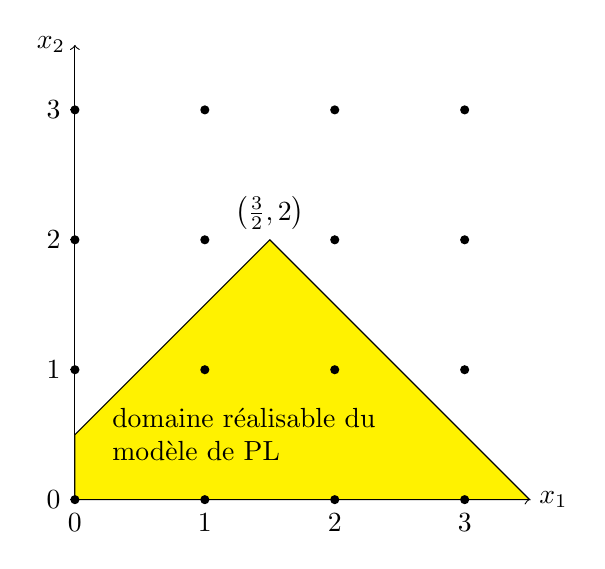
\begin{tikzpicture}[scale=1.65]
\draw[->] (0,0) -- (3.5,0) node[below,right] {$x_1$};
\draw[->] (0,0) -- (0,3.5) node[above,left] {$x_2$};

\foreach \x in {0,1,2,3}
\draw (\x,1pt) -- (\x,-1pt) node[anchor=north] {$\x$};
\foreach \y in {0,1,2,3}
\draw (1pt,\y) -- (-1pt,\y) node[anchor=east] {$\y$};

\filldraw[fill=yellow]
(0,0) -- (0,0.5) -- (1.5,2) -- (3.5,0) -- (0,0);

\draw (1.5,0.5) node[text width=4cm,text ragged] {domaine réalisable du modèle de PL};

\draw (1.5,2) node[above]{$\left( \frac{3}{2},2\right)$};

\foreach \x in {0,1,2,3}
\foreach \y in {0,1,2,3}
\fill (\x,\y) circle (1 pt);;
\end{tikzpicture}
\end{center}

\end{frame}

\begin{frame}
\frametitle{Exemple 2}

Considérons le programme
\begin{align*}
\max\ & z = x_1+5x_2\\
\st & x_1+10x_2 \leq 21, \\
& x_2 \leq 2, \\
& x_1, x_2 \geq 0 \mbox{ et entiers}.
\end{align*}
La version relâchée de programme est
\begin{align*}
\max\ & z = x_1+5x_2\\
\st & x_1+10x_2 \leq 21, \\
& x_2 \leq 2, \\
& x_1, x_2 \geq 0,
\end{align*}
qui a pour solution optimale $(2, 1.9)$. En arrondissant à $(2,1)$ afin de garantir l'admissibilité, nous obtenons la valeur 7 pour la fonction objectif, loin de la valeur optimale du PLNE, avec pour valeur optimale de 11, en $(1,2)$.

\end{frame}

\begin{frame}
\frametitle{Exemple 2}

\begin{center}
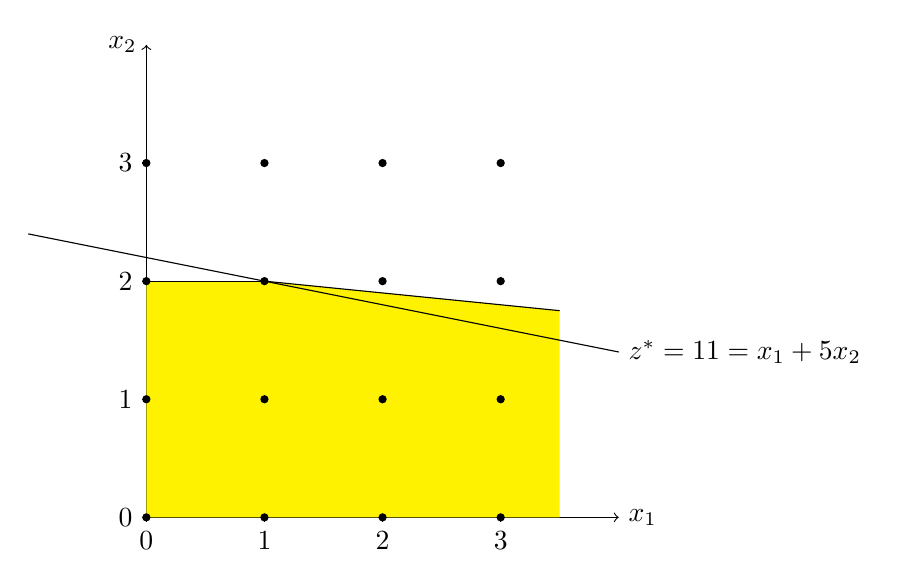
\begin{tikzpicture}[scale=1.50]
\draw[->] (0,0) -- (4,0) node[below,right] {$x_1$};
\draw[->] (0,0) -- (0,4) node[above,left] {$x_2$};

\foreach \x in {0,1,2,3}
\draw (\x,1pt) -- (\x,-1pt) node[anchor=north] {$\x$};
\foreach \y in {0,1,2,3}
\draw (1pt,\y) -- (-1pt,\y) node[anchor=east] {$\y$};

%\filldraw[fill=yellow]
\fill[fill=yellow]
(0,0) -- (0,2) -- (1, 2) -- (3.5,1.75) -- (3.5,0) -- (0,0);
\draw (0, 2) -- (1,2);
\draw (1, 2) -- (3.5,1.75);

\draw (-1,2.4) -- (4,1.4) node[above,right,sloped] {$z^* = 11 = x_1+5x_2$};

\foreach \x in {0,1,2,3}
\foreach \y in {0,1,2,3}
\fill (\x,\y) circle (1 pt);;
\end{tikzpicture}
\end{center}

\end{frame}

\begin{frame}
\frametitle{Approche par énumération}

\begin{itemize}
	\item 
Un modèle en nombres entiers borné (p.e. avec uniquement des variables 0--1) possède un nombre fini de solutions.
	\item 
Nous pourrions envisager de toutes les énumérer, mais le nombre de solutions explose rapidement. Pour $n = 20$ variables 0--1, il y a plus d'un million de solutions possibles.
Pour $n=30$, c'est plus d'un milliard.
	\item 
Énumération complète des solutions: vite déraisonnable .
\end{itemize}

Alternative: \textcolor{red}{énumération partielle}
\begin{itemize}
	\item 
Cette technique est connue sous le vocable de {\sl branch-and-bound} (B\&B).
Il s'agit d'une approche {\sl diviser-pour-régner}:
\begin{itemize}
\item
décomposition du problème en sous-problèmes plus simples;
\item
combinaison de la résolution de ces sous-problèmes pour obtenir la solution du problème original.
\end{itemize}
\end{itemize}

\end{frame}

\begin{frame}
\frametitle{Algorithme de branch-and-bound}

\begin{itemize}
	\item 
Construction d'un arbre de solutions, où chaque sous-problème correspond à un sommet.
\item 
Nous résolvons la relaxation linéaire de chaque sous-problème.
L'information tirée de la relaxation linéaire nous permettra (peut-être) d'éliminer toutes les solutions pouvant être obtenues à partir de ce sommet.
\end{itemize}

\end{frame}

\begin{frame}
\frametitle{Algorithme de branch \& bound: cas 0--1}

Un algorithme simple pour énumérer toutes les solutions d'un modèle 0--1 consiste à:
\begin{itemize}
\item
choisir un sommet dans l'arbre des solutions;
\item
choisir une variable $x$ non encore fixée relativement à ce sommet;
\item
générer les deux variables $x = 0$ et $x = 1$ (la variable $x$ est dite {\sl fixée}): chaque alternative correspond à un sommet de l'arbre des solutions;
\item
recommencer à partir d'un sommet pour lequel certaines variables ne sont pas encore fixées.
\end{itemize}

\end{frame}

\begin{frame}
\frametitle{Algorithme de branch \& bound: cas 0--1}

\begin{itemize}
	\item 
Racine de l'arbre: aucune variable fixée;
\item
Feuilles de l'arbre: toutes les variables sont fixées.\\
Le nombre maximal de feuilles est $2^n$ (pour $n$ variables 0--1).
\end{itemize}

\mbox{}

Le calcul de borne (ou évaluation) consiste à résoudre la relaxation linéaire en chaque sommet.
L'élagage (ou élimination) consiste à utiliser l'information tirée de la résolution de la relaxation linéaire pour éliminer toutes les solutions émanant du sommet courant.
Dès lors, le branch-and-bound est un algorithme de séparation et d'évaluation successives.

\end{frame}

\begin{frame}
\frametitle{Exemple: California Mfg}

Rappelons le problème
\begin{align*}
\min\ & z = -9x_1 -5x_2 -6x_3 -4x_4 \\
\st & 6x_1 + 3x_2 + 5x_3 + 2x_4 \leq 10; \\
& x_3 + x_4 \leq 1; \\
& -x_1 + x_3 \leq 0; \\
& -x_2 + x_4 \leq 0; \\
& x_1, x_2, x_3, x_4 \leq 1; \\
& x_1, x_2, x_3, x_4 \geq 0; \\
& x_1, x_2, x_3, x_4 \mbox{ entiers}.
\end{align*}
La relaxation linéaire permet aux variables de prendre les valeurs fractionnaires entre 0 et 1, ce qui conduit à la solution
\[
\left( \frac{5}{6}, 1, 0, 1 \right),
\]
avec comme valeur $z = -16,5$.
Branchons sur $x_1$.

\end{frame}

\begin{frame}
\frametitle{Exemple: California Mfg}

Dénotons sous-problème 1 celui obtenu avec $x_1 = 0$:
\begin{align*}
\min\ & z = -5x_2 -6x_3 -4x_4 \\
\st & 3x_2 + 5x_3 + 2x_4 \leq 10; \\
& x_3 + x_4 \leq 1; \\
& x_3 \leq 0; \\
& -x_2 + x_4 \leq 0; \\
& x_2, x_3, x_4 \mbox{ binaires}.
\end{align*}
La solution de la relaxation linéaire est $(x_1, x_2, x_3, x_4) = (0,1,0,1)$, avec $z = -9$.

\end{frame}

\begin{frame}
\frametitle{Exemple: California Mfg}

Le sous-problème 2 est celui obtenu avec $x_1 = 1$:
\begin{align*}
\min\ & z = -5x_2 -6x_3 -4x_4 -.. 9 \\
\st & 3x_2 + 5x_3 + 2x_4 \leq 4; \\
& x_3 + x_4 \leq 1; \\
& x_3 \leq 1; \\
& -x_2 + x_4 \leq 0; \\
& x_2, x_3, x_4 \mbox{ binaires}.
\end{align*}
La solution de la relaxation linéaire est alors
\[
(x_1, x_2, x_3, x_4) = \left( 1, \frac{4}{5},0, \frac{4}{5} \right),
\]
avec $z = -16-\frac{1}{5}$.

\end{frame}

\begin{frame}
\frametitle{Exemple: California Mfg}

Nous obtenons dès lors les bornes suivantes:
\begin{itemize}
\item
sous-problème 1: $Z_1 \geq -9$;
\item
sous-problème 2: $Z_2 \geq -16-\frac{1}{5}$.
\end{itemize}

\mbox{}

\begin{itemize}
	\item 
Toutes les variables sont binaires et tous les paramètres dans l'objectif sont des valeurs entières. Dès lors, $Z_2 \geq -16$.
\item 
Pour le sous-problème 1, la solution obtenue est entière: c'est la meilleure solution courante, de valeur objectif notée $Z^*$, et la valeur optimale cherchée, $Z$, satisfait $Z \leq Z^* = -9$.
\end{itemize}

\mbox{}

Quels sous-problèmes pouvons-nous à présent considérer afin de nous approcher de la solution optimale? Tous les sous-problèmes actuellement traités doivent-ils donner naissance à d'autres problèmes?

\end{frame}

\begin{frame}
\frametitle{Exemple: California Mfg}

Si un sous-problème ne donne lieu à aucun autre problème, nous parlerons d'\textcolor{red}{élagage}, en référence avec l'idée de couper la branche correspondante dans l'arbre d'exploration.

\mbox{}

Considérons le sous-problème 1: la solution optimale de la relaxation PL est entière.
Il ne sert à rien de brancher sur les autres variables, puisque toutes les autres solutions entières (avec $x_1 = 0$) sont nécessairement de valeurs supérieures ou égales à -9.
Nous pouvons donc élaguer ce sommet.

\mbox{}

Pour le sous-problème 2, la solution optimale de la relaxation PL n'est pas entière:
$$
Z^* = -9 \geq Z \geq -16.
$$
La branche ($x_1 = 1$) peut encore contenir une solution optimale.
Mais si nous avions eu $Z_2 \geq Z^*$, nous aurions pu conclure que la
branche ne pouvait améliorer la meilleure solution courante.

\end{frame}

\begin{frame}
\frametitle{Élagage}

Un sous-problème est elagué si une des trois conditions suivantes est satisfaite :
\begin{itemize}
\item
\textcolor{blue}{test 1}: sa borne inférieure (valeur optimale de la relaxation PL) est supérieure ou égale à $Z^*$ (valeur de la meilleure solution courante);
\item
\textcolor{blue}{test 2}: sa relaxation PL n'a pas de solution réalisable;
\item
\textcolor{blue}{test 3}: la solution optimale de sa relaxation PL est entière.
\end{itemize}
Lorsque le test 3 est verifié, nous testons si la valeur optimale de la relaxation PL du sous-problème, $Z_i$, est inférieure à $Z^*$.
Si $Z_i < Z^*$, alors $Z^* := Z_i$, et nous conservons la solution, qui
devient la meilleure solution courante.
%En résumé, nous obtenons l'algorithme ci-dessous.

\end{frame}

\begin{frame}
\frametitle{Algorithme branch-and-bound: cas binaire}

\begin{enumerate}
\item
Initialisation:
\begin{enumerate}[(a)]
\item
$Z^* := +\infty$;
\item
appliquer le calcul de borne et les critères d'élagage à la racine (aucune variable fixée).
\end{enumerate}
\item
Arrêt si aucun sous-probleme non élagué.
\item
Branchement:
\begin{enumerate}[(a)]
\item
parmi les sous-problèmes non encore élagués, choisir celui qui a été crée le plus récemment (s'il y a égalité, choisir celui de plus petite borne inférieure);
\item
appliquer le Test 1: si le sous-problème est élagué,
retourner en 2.
\item
brancher sur la prochaine variable non fixée.
\end{enumerate}
\end{enumerate}

\end{frame}

\begin{frame}
\frametitle{Algorithme branch-and-bound: cas binaire}

\begin{enumerate}
\setcounter{enumi}{3}
\item
Calcul de borne:
\begin{enumerate}[(a)]
	\item
	résoudre la relaxation PL de chaque sous-problème;
	\item
	arrondir (vers le haut) la valeur optimale si tous les paramètres de l'objectif sont entiers.
\end{enumerate}
\item
Élaguer un sous-problème si le test 1, 2 ou 3 est satisfait. Si le test 3 est vérifié (solution optimale de la relaxation PL est entière) ET la borne inférieure est strictement inférieure à $Z^*$, $Z^*$ est mise à jour et la solution de la relaxation PL devient la meilleure solution courante.

Retour en 2.
\end{enumerate}

\end{frame}

\begin{frame}
\frametitle{Branchement}

Plusieurs choix possibles du n\oe{}ud duquel brancher.

\mbox{}

\begin{enumerate}
	\item 
\textcolor{blue}{Sous-problème le plus récemment créé}: facilite la réoptimisation lors du calcul de borne, car il n'y a que peu de changements apportés par rapport au dernier sous-problème traité.
Le désavantage est que cela peut créer un grand nombre de sous-problèmes.
	\item 
\textcolor{blue}{Règle de la meilleure borne}: choisir le sous-problème ayant la plus petite borne inférieure.
	\item 
\textcolor{blue}{Prochaine variable non fixée}.
\end{enumerate}

\end{frame}

\begin{frame}
\frametitle{Branchement}

Dans la version retenue ici, la règle de branchement consiste à choisir la prochaine variable non fixée. Il est souvent plus intéressant de choisir une variable à valeur fractionnaire.
En branchant sur une telle variable, il est certain que les deux sous-problèmes créés mènent à des solutions différentes de la solution courante.
De nombreux autres critères existent de facon à orienter la recherche vers un élagage rapide.

\end{frame}

\begin{frame}
\frametitle{Exemple: suite}

Jusqu'à maintenant, voici l'arbre obtenu, en branchant sur la variable $x_1$.
\begin{center}
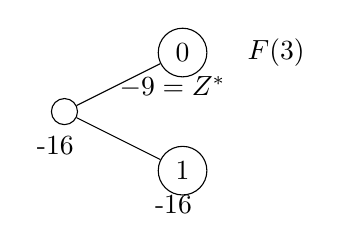
\begin{tikzpicture}
\node (root) [circle,draw] {} [grow'=right]
child {node (A) [circle,draw] {0}}
child {node (B) [circle,draw] {1}};
\draw (root) node[below, text width=7mm, text ragged]{\hspace{5mm} -16}; 
\draw (B) node[below, text width=7mm, text ragged]{\hspace{5mm} -16}; 
\draw (A) node[below, text width=16mm, text ragged]{\hspace{12mm} $-9 = Z^*$}; 
\draw (A) node[right] {\qquad $F(3)$};
\end{tikzpicture}
\end{center}
$F(3)$ indique que le sous-probleme a été élagué ({\sl fathomed}) en raison du Test 3.

\mbox{}

Sélection: nous choisissons le sous-problème 2, le seul qui n'a pas encore été élagué.
Nous branchons sur la prochaine variable, soit $x_2$.
Deux nouveaux sous-problèmes sont créés:
\begin{itemize}
\item
sous-problème 3: $x_1 = 1$, $x_2 = 0$;
\item
sous-problème 4: $x_1 = 1$, $x_2 = 1$.
\end{itemize}

\end{frame}

\begin{frame}
\frametitle{Exemple: sous-problème 3}

$x_1 = 1$, $x_2 = 0$. Sous-problème:
\begin{align*}
\min z_3 =\ & -6x_3 -4x_4 -9 \\
\st{} & 5 x_3 + 2x_4 \leq 4 \\
& x_3 + x_4 \leq 1 \\
& x_3 \leq 1 \\
& x_4 \leq 0 \\
& x_3,\ x_4 \mbox{ binaires}.
\end{align*}
La solution de la relaxation PL est
\[
( x_1, x_2, x_3, x_4) = \left(1,0, \frac{4}{5},0 \right),
\]
et
\[
Z = -13-\frac{4}{5};\ Z_3 \geq -13.
\]

\end{frame}

\begin{frame}
\frametitle{Exemple: sous-problème 4}

$x_1 = 1$, $x_2 = 1$. Sous-problème:
\begin{align*}
\min z_4 =\ & -6x_3 -4x_4 -14 \\
\st{} & 5 x_3 + 2x_4 \leq 1 \\
& x_3 + x_4 \leq 1 \\
& x_3 \leq 1 \\
& x_4 \leq 1 \\
& x_3,\ x_4 \mbox{ binaires}.
\end{align*}
La solution de la relaxation PL est
\[
( x_1, x_2, x_3, x_4) = \left(1,1,0, \frac{1}{2} \right).
\]
et
\[
Z = -16;\ Z_4 \geq -16.
\]

\end{frame}

\begin{frame}
\frametitle{Exemple: suite}

Aucun des tests d'élagage ne s'applique sur ces deux sous-problèmes.
Nous en choisissons un pour effectuer un branchement, puisque ce sont ceux créés le plus récemment.
Nous prenons celui de plus petite borne inférieure, soit le sous-problème 4.

\mbox{}

Deux possibilités existent:
\begin{itemize}
	\item brancher sur la variable fractionnaire, $x_4$,
	\item ou choisir la prochaine variable non fixée, $x_3$.
\end{itemize}
Nous explorons la deuxième approche: nous branchons sur $x_3$.

\end{frame}

\begin{frame}
\frametitle{Exemple: sous-problème 5}

$x_1 = 1$, $x_2 = 1$, $x_3 = 0$. Sous-problème:
\begin{align*}
\min z_5 =\ & -4x_4 - 14 \\
\st{} & 2x_4 \leq 1 \\
& x_4 \leq 1 \\
& x_4 \leq 1 \\
& x_4 \mbox{ binaire}.
\end{align*}

La solution de la relaxation PL est
\[
( x_1, x_2, x_3, x_4) = \left(1,1,0, \frac{1}{2} \right)
\]
et
\[
Z = -16:\ Z_5 \geq -16.
\]

\end{frame}

\begin{frame}
\frametitle{Exemple: sous-problème 6}

$x_1 = 1$, $x_2 = 1$, $x_3 = 1$. Sous-problème:
\begin{align*}
\min z_5 =\ & -4x_4 - 20 \\
\st{} & 2x_4 \leq -1 \\
& x_4 \leq 0 \\
& x_4 \leq 1 \\
& x_4 \mbox{ binaire}.
\end{align*}
Pas de solution réalisable: ce sous-problème est élagué.

\end{frame}

\begin{frame}
\frametitle{Exemple: suite}

Le sous-problème 5 ne peut pas être élagué.
Il est créé le plus récemment parmi les sous-problèmes non élagués (3 et 5); nous le choisissons pour effectuer un branchement.
En branchant sur $x_4$, nous générons
\begin{itemize}
\item
sous-problème 7: $x_1 = 1$, $x_2 = 1$, $x_3 = 0$, $x_4 = 0$;
\item
sous-problème 8: $x_1 = 1$, $x_2 = 1$, $x_3 = 0$, $x_4 = 1$.
\end{itemize}

\mbox{}

Toutes les variables sont fixées.
\begin{itemize}
	\item 
Le sous-problème 7 a pour solution $(x_1, x_2, x_3, x_4) = (1, 1, 0, 0)$, pour $Z_7 = -14$.
Élagage en vertu du Test 3 (solution entière).
Puisque $Z_7 < Z^*$, $Z^* := -14$ et $(1, 1, 0, 0)$ devient la meilleure solution courante.
	\item 
La solution du sous-problème 8 est $(1, 1, 0, 1)$, non-réalisable réalisable, car la première contrainte $(2x_4 \leq 1)$ est violée. Élagage en vertu du Test 2.
\end{itemize} 

\end{frame}

\begin{frame}
\frametitle{Exemple: sous-problème 3 et fin}

Le sous-problème 3 est le seul non encore élagué.

\mbox{}

Nous l'élaguons suite à l'application du Test 1: $Z_3 = -13 \geq -14 = Z*$.

\mbox{}

Arrêt: il n'y a plus de sous-problèmes non élagués.
$$
x^* = (1,1,0,0),\qquad Z^* = -14.
$$

\end{frame}

\begin{frame}
\frametitle{Exemple: arbre}

L'arbre obtenu suite à l'exécution de l'algorithme se présente comme suit:
\begin{center}
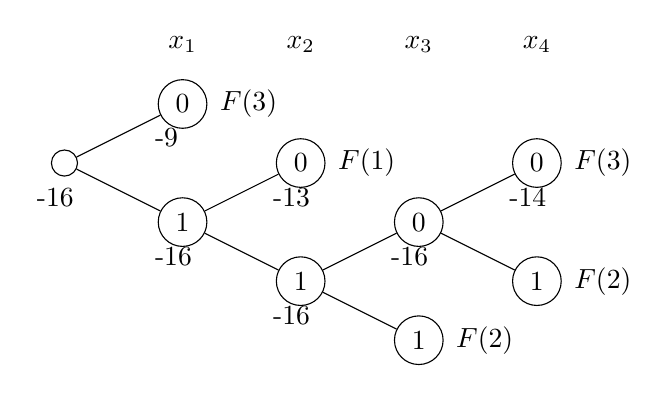
\begin{tikzpicture}
\node (root) [circle,draw] {} [grow'=right]
child {node (A) [circle,draw] {0}}
child {node (B) [circle,draw] {1}
child {node (C) [circle,draw] {0}}
child {node (D) [circle,draw] {1}
child {node (E) [circle,draw] {0}
child {node (F) [circle,draw] {0}}
child {node (G) [circle,draw] {1}}
}
child {node (H) [circle,draw] {1}}
}
};
\draw (root) node[below, text width=7mm, text ragged]{\hspace{5mm} -16}; 
\draw (B) node[below, text width=7mm, text ragged]{\hspace{5mm} -16}; 
\draw (A) node[below, text width=7mm, text ragged]{\hspace{5mm} -9}; 
\draw (D) node[below, text width=7mm, text ragged]{\hspace{5mm} -16}; 
\draw (C) node[below, text width=7mm, text ragged]{\hspace{5mm} -13}; 
\draw (E) node[below, text width=7mm, text ragged]{\hspace{5mm} -16}; 
\draw (F) node[below, text width=7mm, text ragged]{\hspace{5mm} -14}; 
\draw (A) node[right] {\quad $F(3)$};
\draw (F) node[right] {\quad $F(3)$};
\draw (C) node[right] {\quad $F(1)$};
\draw (G) node[right] {\quad $F(2)$};
\draw (H) node[right] {\quad $F(2)$};
\draw (1.5,1.5) node {$x_1$};
\draw (3,1.5) node {$x_2$};
\draw (4.5,1.5) node {$x_3$};
\draw (6,1.5) node {$x_4$};
\end{tikzpicture}
\end{center}
$F(j)$: le sous-problème est élagué par le Test j

\end{frame}

\begin{frame}
\frametitle{Algorithme de branch \& bound: cas général}

\begin{itemize}
	\item 
\textcolor{red}{Programmation (mixte) en nombres entiers}: variables entières générales et variables continues.
	\item 
\textcolor{blue}{Relaxation linéaire}: ignorons les contraintes d'intégralité (les valeurs des variables entières sont traitées comme variables continues), et résolvons le PL résultant.
	\item 
Si la solution optimale du PL satisfait aux contraintes d'intégralité, alors cette solution est aussi solution optimale du programme avec variables entières.
Sinon, il doit exister au moins une variable $x_j$ dont la valeur $\alpha$ est fractionnaire.
\end{itemize}

\end{frame}

\begin{frame}
\frametitle{Algorithme de branch \& bound: cas général}

Soit $d \in \mathbb{R}$. Dénotons $\lfloor d \rfloor$ le plus grand entier tel que $\lfloor d \rfloor \leq d$.

\mbox{}

\textcolor{blue}{Procédure de branchement} nous séparons alors le problème relaxé en deux sous-problèmes:
\begin{itemize}
	\item 
un sous-problème contiendra la contrainte $x_j \leq \lfloor \alpha \rfloor$;
\item
ajouter au second la contrainte $x_j \geq \lceil \alpha \rceil  = \lfloor \alpha \rfloor + 1$.
\end{itemize}
Nous répétons le processus pour chacun des sous-problèmes.

\mbox{}

Cette procédure est habituellement représentée sous forme
d'un arbre binaire où, à chaque niveau, une partition du sommet père s'effectue suivant la règle décrite précédemment.

\mbox{}

Il s'agit alors de parcourir cet arbre d'énumération afin d'y trouver la solution optimale.

\end{frame}

\begin{frame}
\frametitle{Algorithme de branch \& bound: cas général}

L'exploration d'un chemin de l'arbre peut prendre fin pour trois raisons:
\begin{enumerate}
\item
la valeur de l'objectif correspondant à la solution optimale du problème relaxé est supérieure (moins bonne) à celle d'une solution admissible connue, possiblement obtenue à un autre sommet de l'arbre.
\item
le domaine admissible d'un sous-problème devient vide;
\item
la solution devient entière.
\end{enumerate}
Dans chacun de ces trois cas on dit que le sommet est sondé, et il est inutile de pousser plus loin dans cette direction.

\mbox{}

L'algorithme s'arrête lorsque tous les sommets sont sondés.
La meilleure solution obtenue au cours du déroulement de l'algorithme est alors l'optimum global de notre problème.

\end{frame}

\begin{frame}
\frametitle{Algorithme de B\&B: cas général}

\begin{enumerate}
\item
Initialisation:
\begin{enumerate}[(a)]
\item
Poser $Z^* = +\infty$.
\item
Appliquer le calcul de borne et les critères d'élagage à la racine (aucune variable fixée).
\item
Si tous les sous-problèmes ont été élagués, arrêt.
\end{enumerate}
\item
Branchement:
\begin{enumerate}[(a)]
\item
Choisir le sous-problème non encore élagué créé le plus récemment. Si égalité, choisir celui de plus petite borne inférieure.
\item
Appliquer le Test 1: si le sous-problème est élagué, retourner en 2.
\item
Brancher sur la prochaine variable entière à valeur non entière dans la relaxation PL.
\end{enumerate}
\item
Calcul de borne: résoudre la relaxation PL de chaque sous-problème.
\end{enumerate}

\end{frame}

\begin{frame}
\frametitle{Algorithme de B\&B: cas général}

\begin{enumerate}
\setcounter{enumi}{3}
\item
Élagage: élaguer un sous-problème si
\begin{enumerate}[(a)]
\item
La borne inférieure est supérieure ou égale à $Z^*$.
\item
La relaxation PL n'a pas de solution réalisable.
\item
Dans la solution optimale de la relaxation PL, toutes les variables entières sont à valeurs entières: si la valeur optimale du sous-problème est strictement inférieure à $Z^*$, $Z^*$ est mise à jour et la solution de la relaxation PL devient la meilleure solution courante.
\end{enumerate}
\item
Retourner en 2.
\end{enumerate}

\end{frame}

\begin{frame}
\frametitle{Exemple}

Considérons le problème
\begin{align*}
		\min_{x_1,x_2} \ & z = -4x_1+x_2 \\
		\mbox{s.à. } & 3x_1 - 2x_2 \leq 14 \\ 
		& x_2 \leq 3 \\
		& 2x_1 - 2x_2 \leq 3 \\
		& x_1 \in \NN, x_2 \in \NN,
\end{align*}

La relaxation linéaire donne
\begin{align*}
	\min_{x_1,x_2} \ & z = -4x_1+x_2 \\
	\mbox{s.à. } & 3x_1 - 2x_2 \leq 14 \\ 
	& x_2 \leq 3 \\
	& 2x_1 - 2x_2 \leq 3 \\
	& x_1 \geq 0, x_2 \geq 0,
\end{align*}

\end{frame}

\begin{frame}
\frametitle{Exemple}

La solution optimale de la RL est $(9/2, 3)$, avec la valeur optimale -15, qui devient la borne inférieure pour le problème de départ.

Nous créons 2 problèmes en ajoutant une des contraintes
\begin{align*}
x_1 &\leq 4 \\
x_1 &\geq 5
\end{align*}

	\begin{center}
	\begin{forest}
		branch and bound,
		where level=1{
			set branch labels={x_1 \leq 4}{}{x_1 \geq 5}{},
		}{
		}
		[\extraprotect{\big($\frac{9}{2}$,3\big)}:S_0:\extraprotect{$-15 \leq z^* \leq +\infty$}
		[:S_1::
		]
		[:S_2::
		]
		]
	\end{forest}
\end{center}

\end{frame}

\begin{frame}
\frametitle{Exemple}

Considérons tout d'abord le problème $S_1$:
	\begin{align*}
		\min_{x_1,x_2} \ & z = -4x_1+x_2 \\
		\mbox{s.à. } & 3x_1 - 2x_2 \leq 14 \\ 
		& x_2 \leq 3 \\
		& 2x_1 - 2x_2 \leq 3 \\
		& x_1 \leq 4 \\
		& x_1 \geq 0, x_2 \geq 0
	\end{align*}

La solution optimale est $(4, 5/2)$ et la valeur optimale est -13,5. Tous les problèmes issus de $S_1$ devront satisfaire $-13 \leq z^*$ en considérant les conditions de variables entières.
	
\end{frame}

\begin{frame}
	\frametitle{Exemple}


	\begin{center}
	\begin{forest}
		branch and bound,
		where level=1{
			set branch labels={x_1 \leq 4}{}{x_1 \geq 5}{},
		}{
		}
		[\extraprotect{\big($\frac{9}{2}$,3\big)}:S_0:\extraprotect{$-15 \leq z^* \leq +\infty$}
		[\extraprotect{\big(4,$\frac{5}{2}$\big)}:S_1:\extraprotect{$-13 \leq z^* \leq +\infty$}:
		]
		[:S_2::
		]
		]
	\end{forest}
\end{center}

\end{frame}

\begin{frame}
	\frametitle{Exemple}
	
	Considérons ensuite le problème $S_2$:
	\begin{align*}
		\min_{x_1,x_2} \ & z = -4x_1+x_2 \\
		\mbox{s.à. } & 3x_1 - 2x_2 \leq 14 \\ 
		& x_2 \leq 3 \\
		& 2x_1 - 2x_2 \leq 3 \\
		& x_1 \geq 5 \\
		& x_1 \geq 0, x_2 \geq 0
	\end{align*}
	
Le problème est alors non réalisable et nous élaguons le n\oe{}ud.
	
\end{frame}

\begin{frame}
\frametitle{Exemple}

	\begin{center}
		\begin{forest}
			branch and bound,
			where level=1{
				set branch labels={x_1 \leq 4}{}{x_1 \geq 5}{},
			}{
			}
			[\extraprotect{\big($\frac{9}{2}$,2\big)}:S_0:\extraprotect{$-15 \leq z^* \leq +\infty$}
			[\extraprotect{\big(4,$\frac{5}{2}$\big)}:S_1:\extraprotect{\tiny{$-13 \leq z^* \leq +\infty$}}:
			]
			[:S_2:\extraprotect{non réalisable}:
			]
			]
		\end{forest}
	\end{center}

\end{frame}

\begin{frame}
	\frametitle{Exemple}

$S_2$ est élagué, mais pas $S_1$. Seule la variable $x_2$ est non entière, aussi nous branchons sur celle-ci, en considérant les contraintes
	\begin{align*}
		x_2 &\leq 2 \\
		x_2 &\geq 3
	\end{align*}
	
	\begin{center}
		\begin{forest}
			branch and bound,
			where level=1{
				set branch labels={x_1 \leq 4}{}{x_1 \geq 5}{},
			}{
				if level=2{
					set branch labels={x_2 \leq 2}{}{x_2 \geq 3}{},
				}{},
			}
			[\extraprotect{\big($\frac{9}{2}$,3\big)}:S_0:\extraprotect{$-15 \leq z^* \leq +\infty$}
			[\extraprotect{\big(4,$\frac{5}{2}$\big)}:S_1:\extraprotect{$-13 \leq z^* \leq +\infty$}:
			[:S_3::]
			[:S_4::]
			]
			[:S_2:\extraprotect{non réalisable}:
			]
			]
		\end{forest}
	\end{center}
	
\end{frame}

\begin{frame}
	\frametitle{Exemple}
	
	Considérons ensuite le problème $S_3$:
	\begin{align*}
		\min_{x_1,x_2} \ & z = -4x_1+x_2 \\
		\mbox{s.à. } & 3x_1 - 2x_2 \leq 14 \\ 
		& x_2 \leq 2 \\
		& 2x_1 - 2x_2 \leq 3 \\
		& x_1 \leq 4 \\
		& x_1 \geq 0, x_2 \geq 0
	\end{align*}
	
	La solution est $(7/2, 2)$, associée à la valeur de l'objecitf $-12$, qui devient la borne inférieure pour les problèmes issus de $S_3$.
	
\end{frame}


\begin{frame}
	\frametitle{Exemple}
	
	Prenons le problème $S_4$:
	\begin{align*}
		\min_{x_1,x_2} \ & z = -4x_1+x_2 \\
		\mbox{s.à. } & 3x_1 - 2x_2 \leq 14 \\ 
		& x_2 \leq 3,\ x_2 \geq 3 \\
		& 2x_1 - 2x_2 \leq 3 \\
		& x_1 \leq 4 \\
		& x_1 \geq 0, x_2 \geq 0
	\end{align*}

Nous en déduisons immédiatement que $x_2^* = 3$, et de là,
$$
x_1^* = \min \{ 20/3, 9/2, 4 \} = 4.
$$
La solution est entière et donc réalisable pour le problème de départ, associée à la valeur de l'objectif -13, borne supérieure sur la valeur optimale. Nous élaguons.

\end{frame}

\begin{frame}
	\frametitle{Exemple}
	
Nous pouvons résumer nos progrès dans l'arbre ci-dessous.
	\begin{center}
		\begin{forest}
			branch and bound,
			where level=1{
				set branch labels={x_1 \leq 4}{}{x_1 \geq 5}{},
			}{
				if level=2{
					set branch labels={x_2 \leq 2}{}{x_2 \geq 3}{},
				}{},
			}
			[\extraprotect{\big($\frac{9}{2}$,3\big)}:S_0:\extraprotect{$-15 \leq z^* \leq +\infty$}
			[\extraprotect{\big(4,$\frac{5}{2}$\big)}:S_1:\extraprotect{$-13 \leq z^* \leq +\infty$}:
			[\extraprotect{\big($\frac{7}{2}$,2\big)}:S_3:\extraprotect{\tiny{$-12 \leq z^* \leq +\infty$}}:]
			[\extraprotect{(4,3)}:S_4:\extraprotect{$-15 \leq z^* \leq -13$}:]
			]
			[:S_2:\extraprotect{non réalisable}:
			]
			]
		\end{forest}
	\end{center}

La borne inférieure sur $S_3$ est supérieure à la borne supérieure sur la valeur optimale. Nous élaguons $S_3$.

\end{frame}

\begin{frame}
\frametitle{Exemple}

Il n'y a plus de n\oe{}ud non élagués. Nous avons donc terminer.

\mbox{}

Solution optimale: $x_1^* = 4$, $x_2^* = 3$.

Valeur optimale: $z^* = -13$.

\end{frame}

\begin{frame}
\frametitle{Méthodes de coupes}

\textcolor{blue}{Principe de base}

\mbox{}

Nous cherchons à générer un ensemble de contraintes
linéaires que nous ajoutons à \eqref{eq:PLNE}
pour engendrer un nouveau
problème restreint (PR) tel que
\begin{align*}
\cF{(PRL)} &\subseteq \cF \eqref{eq:PL} \\
\cF{(PR)} &= \cF\eqref{eq:PLNE}
\end{align*}
où (PRL) désigne la relaxation linéaire du problème restreint.

\mbox{}

But: si suffisamment de coupes sont ajoutées, en résolvant le problème relaxé, la solution optimale est entière et donc optimale pour \eqref{eq:PLNE}.

\end{frame}

\begin{frame}
\frametitle{Exemple}

Considérons le programme
\begin{align*}
	\max\ & z = x_1+5x_2\\
	\st & x_1+4x_2 \leq 8,4, \\
	& x_1 \leq 2, \\
	& x_1, x_2 \geq 0 \mbox{ et entiers}.
\end{align*}
Ajoutons la contrainte $x_1 + 2x_2 \leq 4$:
\begin{align*}
	\max\ & z = x_1+5x_2\\
	\st & x_1+4x_2 \leq 8,4, \\
	& x_1 \leq 2, \\
	& x_1 + 2x_2 \leq 4, \\
	& x_1, x_2 \geq 0 \mbox{ et entiers}.
\end{align*}

\end{frame}

\begin{frame}
\frametitle{Exemple}

\begin{center}
	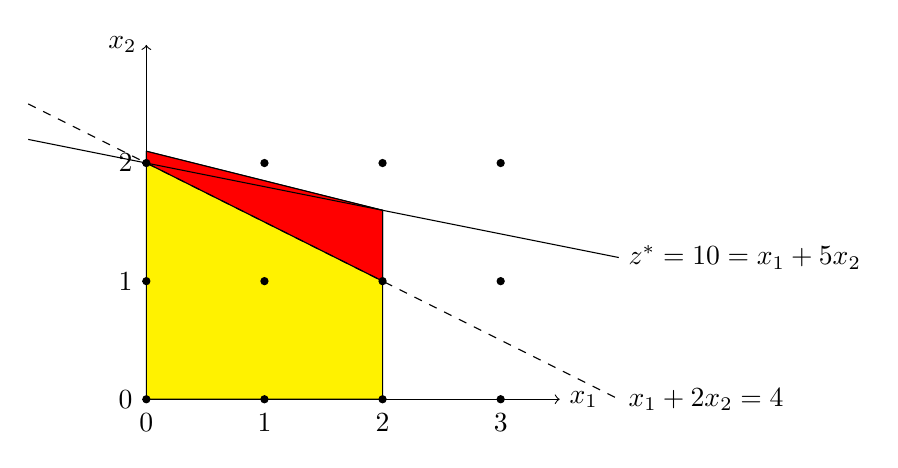
\begin{tikzpicture}[scale=1.50]
		\draw[->] (0,0) -- (3.5,0) node[below,right] {$x_1$};
		\draw[->] (0,0) -- (0,3) node[above,left] {$x_2$};
		
		\foreach \x in {0,1,2,3}
		\draw (\x,1pt) -- (\x,-1pt) node[anchor=north] {$\x$};
		\foreach \y in {0,1,2}
		\draw (1pt,\y) -- (-1pt,\y) node[anchor=east] {$\y$};
		
\filldraw[fill=yellow]
(0,0) -- (0,2.1) -- (2,1.6) -- (2,0) -- (0,0);

%		\filldraw[fill=yellow]
%		(0,0) -- (0,2) -- (2,1.8) -- (2,0) -- (0,0);
		
		\filldraw[fill=red]
		(0,2.1) -- (0,2) -- (2,1) -- (2,1.6) -- (0,2.1);

		\draw (-1,2.2) -- (4,1.2) node[above,right,sloped] {$z^* = 10 = x_1+5x_2$};
		\draw [dashed](-1,2.5) -- (4,0) node[above,right,sloped] {$x_1 + 2x_2 = 4$};
		
		\foreach \x in {0,1,2,3}
		\foreach \y in {0,1,2}
		\fill (\x,\y) circle (1 pt);;
	\end{tikzpicture}
\end{center}

\end{frame}

\begin{frame}
\frametitle{Méthode des coupes de Gomory}

\begin{itemize}
	\item 
\textcolor{blue}{Principe des méthodes de coupes:}
ajouter de nouvelles contraintes linéaires d'inégalité au problème pour
réduire le domaine réalisable du problème relaxé sans pour
autant éliminer de points du domaine réalisable du problème
avec les contraintes de nombre entier sur les variables.
Une telle contrainte est une \textcolor{red}{coupe valide}.
	\item 
La procédure consiste à résoudre une suite de problèmes
relaxés jusqu’à ce qu’une solution optimale en nombres entiers
soit obtenue.
	\item 
Un problème de la suite est obtenu du précédent en lui ajoutant
une contrainte linéaire (coupe) supplémentaire.
\end{itemize}

\end{frame}

\begin{frame}
\frametitle{Construction des coupes}

Reprenons le problème
\begin{equation}
	\begin{aligned}
		\min\ & c^Tx \\
		\mbox{s.à } & Ax = b \\
		& x_i \in \mathbb{N},\ i = 1,\ldots,n.
	\end{aligned}
	\tag{P}
\end{equation}

\mbox{}

Soit $B$ une base optimale de \eqref{eq:PL}, et $x_k$ la variable de base dans la $i^e$ ligne du tableau optimal prenant une valeur qui n'est pas entière.

\end{frame}

\begin{frame}
\frametitle{Construction des coupes}

Le tableau optimal du simplexe du problème relaxé est alors de la forme
\begin{footnotesize}
$$
\begin{array}{c|ccccccccccc|c}
& x_1 & \ldots & x_k & \ldots & x_{j_1}& \ldots & x_j & \ldots & x_{j_m} & \ldots & x_n & \\
\hline
x_{j_1}& y_{1,1} & \ldots & 0 & \ldots & 1 & \ldots & y_{1,j} & \ldots & 0 & \ldots & y_{1,n} & y_{1,0} \\
\vdots & \vdots & \ddots & \vdots & \ddots & \vdots & \ddots & \vdots & \ddots & \vdots & \ddots & \vdots & \vdots \\
x_k & y_{i,1} & \ldots & 1 & \ldots & 0 & \ldots & y_{i,j} & \ldots & 0 & \ldots & y_{i,n} & y_{i,0} \\
\vdots & \vdots & \ddots & \vdots & \ddots & \vdots & \ddots & \vdots & \ddots & \vdots & \ddots & \vdots & \vdots \\
x_{j_m} & y_{m,1} & \ldots & 0 & \ldots & 0 & \ldots & y_{m,j} & \ldots & 1 & \ldots & y_{m,n} & y_{m,0} \\
\hline
& r_1 & \ldots & 0 & \ldots & 0 & \ldots & r_j & \ldots & 0 & \ldots & r_n & -z_0
\end{array}
$$
\end{footnotesize}

La ligne correspondante dans le tableau final du simplexe est
$$
x_k + \sum_{j \in J} y_{i,j}x_j = y_{i,0},
$$
où $y_{i,0} \in \mathbb{R}^+ \setminus \mathbb{N}$ et $J$ est l'ensemble des indices des variables hors base.

\end{frame}

\begin{frame}
\frametitle{Construction des coupes}

Du tableau du simplexe,
\begin{equation}
x_k + \sum_{j \in J} y_{i,j}x_j = y_{i,0}.
\label{eq:cut1}
\end{equation}
Comme $x \geq 0$, nous avons aussi
$$
x_k + \sum_{j \in J} \lfloor y_{i,j} \rfloor x_j \leq y_{i,0}
$$
et si $x$ satisfait les contraintes d'intégralité,
\begin{equation}
x_k + \sum_{j \in J} \lfloor y_{i,j} \rfloor x_j \leq \lfloor y_{i,0} \rfloor.
	\label{eq:cut2}
\end{equation}
Cette dernière inégalité doit être satisfaite $\forall x \in \cF(\ref{eq:PLNE})$, comme par rapport à la base $B$, les contraintes linéaires peuvent se réécrire $B^{-1}Ax = B^{-1}b = y$.
%De plus, comme $\cF{\eqref{eq:PLNE}} \subset \cF{\eqref{eq:PL}}$.

\end{frame}

\begin{frame}
\frametitle{Construction des coupes}

En soustrayant \eqref{eq:cut1} de \eqref{eq:cut2}, nous  obtenons que si $x \in \cF(\ref{eq:PLNE})$,
$$
\sum_{j \in J} \left( \lfloor y_{i,j} \rfloor - y_{i,j} \right) x_i \leq \lfloor y_{i,0} \rfloor - y_{i,0}.
$$
L'introduction de cette contrainte dans \eqref{eq:PLNE} n'élimine donc aucune solution de \eqref{eq:PLNE}.

\mbox{}

Par contre, la solution actuelle du problème relaxé $\eqref{eq:PL}$ ne satisfait pas cette inégalité, et est rejetée en l'incluant dans le problème. En effet, la solution actuelle a comme composante $x_k = y_{i,0} > \lfloor y_{i,0} \rfloor$, et $x_j = 0, j \in J$.

\end{frame}

\begin{frame}
\frametitle{Retour au simplexe}

Pour poursuivre la résolution, il suffit d'introduire la contrainte
$$
\sum_{j \in J} \left( \lfloor y_{i,j} \rfloor - y_{i,j} \right) x_j \leq \lfloor y_{i,0} \rfloor - y_{i,0}.
$$
qui revient à
$$
\sum_{j \in J} \left( \lfloor y_{i,j} \rfloor - y_{i,j} \right) x_j + s_{\tau} = \lfloor y_{i,0} \rfloor - y_{i,0}.
$$
où $s_{\tau}$ est une variable d'écart avec coût nul.

\mbox{}

Cette contrainte est ajoutée au dernier tableau du simplexe pour générer une solution de base au nouveau problème en considérant $s_{\tau}$ comme la variable de base dans la nouvelle ligne du tableau.
Cette solution de base n'est pas réalisable puisque
$$
s_{\tau} = \lfloor y_{i,0} \rfloor - y_{i,0} < 0.
$$

\end{frame}

\begin{frame}
\frametitle{Tableau du simplexe}

\begin{footnotesize}
	$$
\arraycolsep=1pt
	\begin{array}{c|cccccccccccc|c}
		& x_1 & \ldots & x_k & \ldots & x_{j_1}& \ldots & x_j & \ldots & x_{j_m} & \ldots & x_n & s_{\tau} \\
		\hline
		x_{j_1}& y_{1,1} & \ldots & 0 & \ldots & 1 & \ldots & y_{1,j} & \ldots & 0 & \ldots & y_{1,n} & 0 & y_{1,0} \\
		\vdots & \vdots & \ddots & \vdots & \ddots & \vdots & \ddots & \vdots & \ddots & \vdots & \ddots & \vdots & \vdots & \vdots \\
		x_k & y_{i,1} & \ldots & 1 & \ldots & 0 & \ldots & y_{i,j} & \ldots & 0 & \ldots & y_{i,n} & 0 & y_{i,0} \\
		\vdots & \vdots & \ddots & \vdots & \ddots & \vdots & \ddots & \vdots & \ddots & \vdots & \ddots & \vdots & \vdots & \vdots \\
		x_{j_m} & y_{m,1} & \ldots & 0 & \ldots & 0 & \ldots & y_{m,j} & \ldots & 1 & \ldots & y_{m,n} & 0 & y_{m,0} \\
		s_{\tau} & \lfloor y_{i,1} \rfloor - y_{i,1} & \ldots & 0 & \ldots & 0 & \ldots & \lfloor y_{i,j} \rfloor - y_{i,j} & \ldots & 1 & \ldots & \lfloor y_{i,n} \rfloor - y_{i,n} & 1 & \lfloor y_{i,0} \rfloor - y_{i,0} \\
		\hline
		& r_1 & \ldots & 0 & \ldots & 0 & \ldots & r_j & \ldots & 0 & \ldots & r_n & 0 & -z_0
	\end{array}
	$$
\end{footnotesize}

\end{frame}

\begin{frame}
\frametitle{Simplexe dual}

Il suffit de poursuivre la résolution avec l'algorithme dual du simplexe.

\mbox{}

\begin{enumerate}
	\item
	Si $\lfloor y_{ij} \rfloor = y_{ij}$, $\forall j \in J$, et si $y_{i0}$ n'est pas entier, alors
    $$
	x_k + \sum_{j \in J} y_{ij} x_j = y_{i0},
	$$
	indique que \eqref{eq:PLNE} n'est pas réalisable puisque le terme de gauche prend une
	valeur entière pour toute solution réalisable de \eqref{eq:PLNE} alors que le terme de
	droite n'est pas entier.
	\item
	Une dérivation similaire s'applique à toutes les itérations.
\end{enumerate}

\end{frame}

\begin{frame}
\frametitle{Exemple 2}

Reprenons à présent l'exemple
\begin{align*}
	\min\ & z = -x_2\\
	\st & -x_1+x_2 \leq \frac{1}{2}, \\
	& x_1 + x_2 \leq \frac{7}{2}, \\
	& x_1, x_2 \geq 0 \mbox{ et entiers}.
\end{align*}

\end{frame}

\begin{frame}
\frametitle{Exemple 2}

Si nous ajoutons l'inégalité $x_2 \leq 1$, nous obtenons le problème
\begin{align*}
	\min\ & z = -x_2\\
	\st & -x_1+x_2 \leq \frac{1}{2}, \\
	& x_1 + x_2 \leq \frac{7}{2}, \\
	& x_2 \leq 1, \\
	& x_1, x_2 \geq 0 \mbox{ et entiers}.
\end{align*}
\end{frame}

\begin{frame}
\frametitle{Exemple}

\begin{center}
	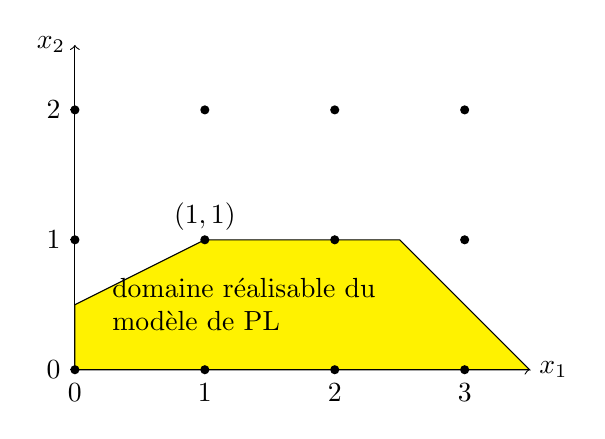
\begin{tikzpicture}[scale=1.65]
		\draw[->] (0,0) -- (3.5,0) node[below,right] {$x_1$};
		\draw[->] (0,0) -- (0,2.5) node[above,left] {$x_2$};
		
		\foreach \x in {0,1,2,3}
		\draw (\x,1pt) -- (\x,-1pt) node[anchor=north] {$\x$};
		\foreach \y in {0,1,2}
		\draw (1pt,\y) -- (-1pt,\y) node[anchor=east] {$\y$};
		
		\filldraw[fill=yellow]
		(0,0) -- (0,0.5) -- (1,1) -- (2.5,1) -- (3.5,0) -- (0,0);
		
		\draw (1.5,0.5) node[text width=4cm,text ragged] {domaine réalisable du modèle de PL};
		
		\draw (1,1) node[above]{$\left( 1, 1 \right)$};
		
		\foreach \x in {0,1,2,3}
		\foreach \y in {0,1,2}
		\fill (\x,\y) circle (1 pt);;
	\end{tikzpicture}
\end{center}

Dans ce cas, le point extrême $(1,1)$ est bien solution, mais il existe d'autres solutions pour le problème relaxé qui ne sont pas entières.

\end{frame}

\end{document}